% =====================================================================
%  MCR2 × NVIDIA  ·  Final Challenge — Week 7
%  Author: Alfonso Diaz
%  Build:  pdflatex presentation.tex (twice)
% =====================================================================
\documentclass[10pt,aspectratio=169]{beamer}

% ---- Clean white theme ----------------------------------------------
\usetheme{default}
\usecolortheme{seahorse}
\setbeamercolor{background canvas}{bg=white}
\setbeamercolor{normal text}{fg=black}
\setbeamercolor{frametitle}{fg=black,bg=white}
\setbeamercolor{title}{fg=black}
\setbeamercolor{structure}{fg=black!75}
\setbeamercolor{itemize item}{fg=black!75}
\setbeamercolor{itemize subitem}{fg=black!60}
\setbeamertemplate{navigation symbols}{}
\setbeamertemplate{itemize item}{\textbullet}
\setbeamertemplate{itemize subitem}{\textendash}
\setbeamerfont{frametitle}{size=\large,series=\bfseries}
\setbeamerfont{title}{size=\Large,series=\bfseries}

% Subtle footer with slide numbers
\setbeamertemplate{footline}{%
  \hbox{%
    \hspace*{1em}\scriptsize\textcolor{black!50}{Alfonso Diaz · MCR2 Final Challenge · Week 7}%
    \hfill\scriptsize\textcolor{black!50}{\insertframenumber\,/\,\inserttotalframenumber}%
    \hspace*{1em}%
  }\vspace*{0.4em}%
}

% ---- Packages -------------------------------------------------------
\usepackage[T1]{fontenc}
\usepackage{lmodern}
\usepackage{amsmath,amssymb,bm}
\usepackage{booktabs}
\usepackage{tikz}
\usetikzlibrary{positioning,arrows.meta,shapes.geometric}
\usepackage{listings}
\usepackage{xcolor}

\lstset{
  basicstyle=\ttfamily\scriptsize,
  keywordstyle=\bfseries,
  commentstyle=\itshape\color{black!55},
  showstringspaces=false,
  frame=single,
  rulecolor=\color{black!20},
  backgroundcolor=\color{black!2},
  breaklines=true,
  language=Python,
}

% ---- Title metadata -------------------------------------------------
\title{Autonomous Puzzlebot Navigation}
\subtitle{EKF Localization with ArUco Markers \& A* Path Planning}
\author{Alfonso Diaz}
\institute{Manchester Robotics × NVIDIA \\ Tecnológico de Monterrey · TE3003B}
\date{Final Challenge · Week 7}

\begin{document}

% =====================================================================
\begin{frame}
  \titlepage
  \vfill
  \begin{center}\small
    \textit{From scratch with NumPy + Python stdlib only}\\[0.3em]
    \textcolor{black!55}{\footnotesize ROS\,2 Humble · Gazebo Harmonic}
  \end{center}
\end{frame}

% =====================================================================
\begin{frame}{Mission}
  \begin{columns}[T,onlytextwidth]
    \column{0.55\textwidth}
    \textbf{Part 1 — EKF Localization}\\[0.3em]
    Estimate the robot pose $(x, y, \theta)$ from wheel encoders
    and ArUco marker observations.
    \medskip

    \textbf{Part 2 — Multi-Waypoint Navigation}\\[0.3em]
    Drive the Puzzlebot through a closed trajectory of
    $\geq 4$ waypoints inside a maze, avoiding walls.
    \medskip

    \textbf{Constraint}\\[0.3em]
    Only \texttt{numpy} + Python stdlib. \\
    No \texttt{scipy}, no Nav2, no SLAM toolbox.
    Everything from scratch.

    \column{0.4\textwidth}
    \centering
    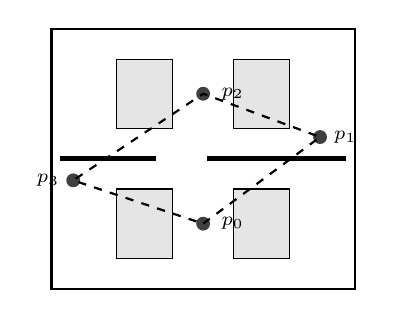
\begin{tikzpicture}[scale=0.55]
      % Outer arena
      \draw[thick] (-1,-1) rectangle (6,5);
      % Inner chambers
      \draw[fill=black!10] (0.5,2.7) rectangle (1.8,4.3);
      \draw[fill=black!10] (3.2,2.7) rectangle (4.5,4.3);
      \draw[fill=black!10] (0.5,-0.3) rectangle (1.8,1.3);
      \draw[fill=black!10] (3.2,-0.3) rectangle (4.5,1.3);
      % Mid divider (gap)
      \draw[line width=2pt] (-0.8,2) -- (1.4,2);
      \draw[line width=2pt] (2.6,2) -- (5.8,2);
      % Waypoints
      \foreach \p/\l in {(2.5,0.5)/p_0,(5.2,2.5)/p_1,(2.5,3.5)/p_2,(-0.5,1.5)/p_3} {
        \fill[black!75] \p circle (0.16);
      }
      \node[anchor=west] at (2.7,0.5) {\scriptsize $p_0$};
      \node[anchor=west] at (5.3,2.5) {\scriptsize $p_1$};
      \node[anchor=west] at (2.7,3.5) {\scriptsize $p_2$};
      \node[anchor=east] at (-0.6,1.5) {\scriptsize $p_3$};
      % Path
      \draw[dashed,thick] (2.5,0.5) -- (5.2,2.5) -- (2.5,3.5) -- (-0.5,1.5) -- (2.5,0.5);
    \end{tikzpicture}
    \par\medskip
    \scriptsize Maze with 4 inner chambers \\ and closed waypoint loop
  \end{columns}
\end{frame}

% =====================================================================
\begin{frame}{System architecture}
  \centering
  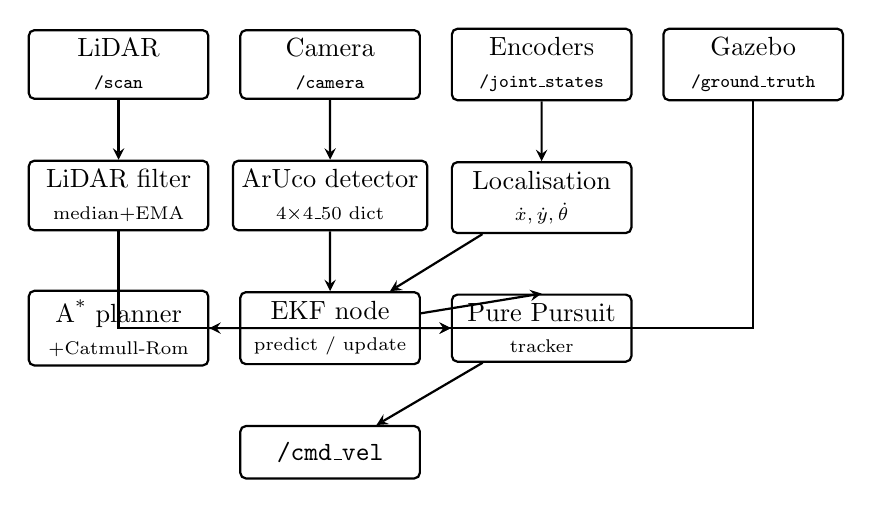
\begin{tikzpicture}[
    box/.style={draw,thick,rounded corners=2pt,minimum width=2.4cm,minimum height=0.7cm,align=center,fill=white},
    arr/.style={-stealth,thick},
    scale=0.95, transform shape
  ]
    % Layer 1: sensors
    \node[box] (lidar) {LiDAR\\\scriptsize\texttt{/scan}};
    \node[box, right=0.4cm of lidar] (cam) {Camera\\\scriptsize\texttt{/camera}};
    \node[box, right=0.4cm of cam] (enc) {Encoders\\\scriptsize\texttt{/joint\_states}};
    \node[box, right=0.4cm of enc] (gz) {Gazebo\\\scriptsize\texttt{/ground\_truth}};

    % Layer 2: perception
    \node[box, below=0.8cm of lidar] (lf) {LiDAR filter\\\scriptsize median+EMA};
    \node[box, below=0.8cm of cam] (ar) {ArUco detector\\\scriptsize 4×4\_50 dict};
    \node[box, below=0.8cm of enc] (loc) {Localisation\\\scriptsize $\dot{x},\dot{y},\dot{\theta}$};

    % Layer 3: estimation + planning
    \node[box, below=0.8cm of ar] (ekf) {EKF node\\\scriptsize predict / update};
    \node[box, left=0.4cm of ekf] (planner) {A\textsuperscript{*} planner\\\scriptsize +Catmull-Rom};
    \node[box, right=0.4cm of ekf] (pp) {Pure Pursuit\\\scriptsize tracker};

    % Layer 4: actuation
    \node[box, below=0.8cm of ekf] (cmd) {\texttt{/cmd\_vel}};

    % Arrows
    \draw[arr] (lidar) -- (lf);
    \draw[arr] (cam) -- (ar);
    \draw[arr] (enc) -- (loc);
    \draw[arr] (ar) -- (ekf);
    \draw[arr] (loc) -- (ekf);
    \draw[arr] (gz) |- (planner);
    \draw[arr] (planner) -- (pp);
    \draw[arr] (ekf) -- (pp.north);
    \draw[arr] (lf) |- (pp);
    \draw[arr] (pp) -- (cmd);
  \end{tikzpicture}
  \par\medskip
  \scriptsize Every block: pure NumPy + ROS\,2 Python. No external planners.
\end{frame}

% =====================================================================
\section{Part 1 — EKF Localization}

\begin{frame}{Differential drive kinematics}
  Wheel velocities $\omega_r, \omega_l$ are read from encoders. Body twist:
  \[
    v = \frac{r}{2}(\omega_r + \omega_l), \qquad
    \omega = \frac{r}{L}(\omega_r - \omega_l)
  \]
  where $r=0.05\,\text{m}$ (wheel radius) and $L=0.19\,\text{m}$ (wheelbase).

  \medskip
  Discrete pose propagation with sample time $\Delta t$:
  \[
    \begin{bmatrix} x_{k+1} \\ y_{k+1} \\ \theta_{k+1}\end{bmatrix}
    = \begin{bmatrix} x_k \\ y_k \\ \theta_k\end{bmatrix}
    + \Delta t \begin{bmatrix} v_k\cos\theta_k \\ v_k\sin\theta_k \\ \omega_k\end{bmatrix}
  \]

  \medskip
  This is the \emph{nominal} motion model — it drifts because of slip, quantization
  and unmodelled dynamics. We need observations to correct it.
\end{frame}

% =====================================================================
\begin{frame}{EKF — Prediction step}
  State $\bm{\mu}_k = [x_k, y_k, \theta_k]^\top$, covariance $\Sigma_k \in \mathbb{R}^{3\times 3}$.

  \medskip
  \textbf{Mean propagation} (nominal kinematics, $f(\bm{\mu}_{k-1}, u_k)$):
  \[
    \bm{\mu}_{k|k-1} = f(\bm{\mu}_{k-1}, u_k)
  \]

  \textbf{Covariance propagation} with Jacobian $F_k = \partial f/\partial \bm{\mu}$:
  \[
    \Sigma_{k|k-1} = F_k\, \Sigma_{k-1}\, F_k^\top + Q_k
  \]
  \[
    F_k = \begin{bmatrix}
      1 & 0 & -\Delta t\, v_k \sin\theta_{k-1} \\
      0 & 1 & \phantom{-}\Delta t\, v_k \cos\theta_{k-1} \\
      0 & 0 & 1
    \end{bmatrix}
  \]

  \textbf{Process noise} $Q_k$ derives from per-wheel proportional noise:
  \[
    Q_k = B_k\, \mathrm{diag}(k_r |\omega_r|,\; k_l |\omega_l|)\, B_k^\top,
    \quad k_r = k_l = 0.15
  \]
\end{frame}

% =====================================================================
\begin{frame}{EKF — Observation model (range-bearing)}
  For ArUco marker $i$ at known map location $(m_x^i, m_y^i)$, the camera measures:
  \[
    z = \begin{bmatrix} r \\ \beta \end{bmatrix} =
    \begin{bmatrix}
      \sqrt{(m_x^i - x)^2 + (m_y^i - y)^2} \\
      \arctan2(m_y^i - y,\; m_x^i - x) - \theta
    \end{bmatrix}
  \]

  \textbf{Measurement Jacobian} $H_k = \partial h / \partial \bm{\mu}$:
  \[
    H_k = \begin{bmatrix}
      -\dfrac{\Delta x}{r} & -\dfrac{\Delta y}{r} & 0 \\[0.6em]
      \phantom{-}\dfrac{\Delta y}{r^2} & -\dfrac{\Delta x}{r^2} & -1
    \end{bmatrix}
  \]
  with $\Delta x = m_x^i - x,\ \Delta y = m_y^i - y$.

  \medskip
  \textbf{Observation noise}: $R = \mathrm{diag}(\sigma_r^2, \sigma_\beta^2)$
  with $\sigma_r = 0.08\,\text{m}$, $\sigma_\beta = 0.06\,\text{rad}\,(\approx 3.5^\circ)$.
\end{frame}

% =====================================================================
\begin{frame}{EKF — Update step \& outlier rejection}
  \textbf{Innovation} $\nu_k$ and its covariance $S_k$:
  \[
    \nu_k = z_k - h(\bm{\mu}_{k|k-1}), \qquad
    S_k = H_k\, \Sigma_{k|k-1}\, H_k^\top + R
  \]
  Wrap the bearing component of $\nu_k$ into $(-\pi,\pi]$ before using it.

  \medskip
  \textbf{Mahalanobis gate} — reject observations with
  \[
    d^2 = \nu_k^\top S_k^{-1} \nu_k > \chi^2_{2,\,0.999} \approx 30
  \]
  protects the filter against false detections / wrong marker IDs.

  \medskip
  \textbf{Kalman gain \& update}:
  \[
    K_k = \Sigma_{k|k-1}\, H_k^\top\, S_k^{-1}
  \]
  \[
    \bm{\mu}_k = \bm{\mu}_{k|k-1} + K_k\,\nu_k, \qquad
    \Sigma_k = (I - K_k H_k)\,\Sigma_{k|k-1}
  \]
\end{frame}

% =====================================================================
\begin{frame}{ArUco map (14 markers)}
  \centering
  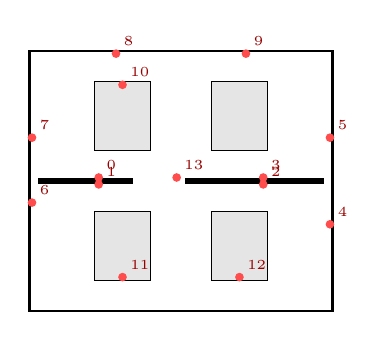
\begin{tikzpicture}[scale=0.55]
    \draw[thick] (-1,-1) rectangle (6,5);
    \draw[fill=black!10] (0.5,2.7) rectangle (1.8,4.3);
    \draw[fill=black!10] (3.2,2.7) rectangle (4.5,4.3);
    \draw[fill=black!10] (0.5,-0.3) rectangle (1.8,1.3);
    \draw[fill=black!10] (3.2,-0.3) rectangle (4.5,1.3);
    \draw[line width=2pt] (-0.8,2) -- (1.4,2);
    \draw[line width=2pt] (2.6,2) -- (5.8,2);
    % Markers — id positions from aruco_map.yaml
    \foreach \id/\x/\y in {1/0.6/1.92, 2/4.4/1.92, 0/0.6/2.08, 3/4.4/2.08,
                            4/5.94/1.0, 5/5.94/3.0, 6/-0.94/1.5, 7/-0.94/3.0,
                            8/1.0/4.94, 9/4.0/4.94, 10/1.15/4.22,
                            11/1.15/-0.22, 12/3.85/-0.22, 13/2.4/2.08} {
      \fill[red!70] (\x,\y) circle (0.10);
      \node[font=\tiny,red!60!black] at (\x,\y) [above right=-1pt] {\id};
    }
  \end{tikzpicture}
  \par\medskip
  \scriptsize 14 markers covering every corridor segment. From any waypoint,
  the robot sees $\geq 2$ markers within 2.5\,m — guaranteed redundancy.
\end{frame}

% =====================================================================
\begin{frame}{Covariance ellipse (visual interpretation)}
  Project the $2\times 2$ XY block of $\Sigma_k$ onto the plane:
  \[
    \Sigma_{xy} = \begin{bmatrix} \sigma_{xx} & \sigma_{xy} \\ \sigma_{xy} & \sigma_{yy}\end{bmatrix},
    \quad \Sigma_{xy} = V\Lambda V^\top
  \]
  with eigenvalues $\Lambda = \mathrm{diag}(\lambda_1, \lambda_2)$ and eigenvectors $V$.

  \medskip
  \textbf{95\% confidence ellipse} (2 dof, $\chi^2 = 5.991$):
  \[
    a = \sqrt{\chi^2 \lambda_{\max}}, \qquad b = \sqrt{\chi^2 \lambda_{\min}}
  \]
  Rotation angle: $\alpha = \arctan2(v_{\max,y},\, v_{\max,x})$.

  \medskip
  In RViz: the ellipse \textbf{grows} on stretches without markers
  (uncertainty accumulates) and \textbf{shrinks} when an ArUco update lands —
  visual proof the filter is working.
\end{frame}

% =====================================================================
\section{Part 2 — Navigation}

\begin{frame}{Occupancy grid \& A\textsuperscript{*} planner}
  \begin{columns}[T,onlytextwidth]
    \column{0.55\textwidth}
    \textbf{Grid build from YAML}: each wall is a rectangle in metric coords.
    Discretized to $140\times120$ cells (resolution 5\,cm).

    \medskip
    \textbf{Configuration-space inflation}: dilate occupied cells by
    $r = 0.28\,\text{m}$ so the planner never produces paths that
    clip a wall.

    \medskip
    \textbf{A\textsuperscript{*}} on 8-connected grid:
    \[
      f(n) = g(n) + h(n), \quad
      h(n) = \sqrt{(x_n - x_g)^2 + (y_n - y_g)^2}
    \]
    Implemented with a binary heap (\texttt{heapq}) — admissible heuristic
    guarantees optimality.

    \column{0.42\textwidth}
    \centering
    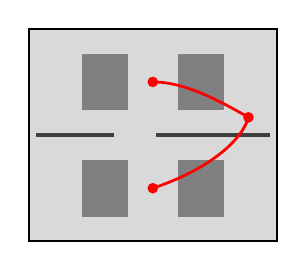
\begin{tikzpicture}[scale=0.45]
      \draw[step=0.2cm,gray!30,very thin] (-1,-1) grid (6,5);
      \draw[thick,fill=black!15] (-1,-1) rectangle (6,5);
      \fill[black!50] (0.5,2.7) rectangle (1.8,4.3);
      \fill[black!50] (3.2,2.7) rectangle (4.5,4.3);
      \fill[black!50] (0.5,-0.3) rectangle (1.8,1.3);
      \fill[black!50] (3.2,-0.3) rectangle (4.5,1.3);
      \fill[black!75] (-0.8,1.94) rectangle (1.4,2.06);
      \fill[black!75] (2.6,1.94) rectangle (5.8,2.06);
      % A* path
      \draw[red,line width=1pt] (2.5,0.5) .. controls (4.0,1.0) and (5.0,1.8) .. (5.2,2.5);
      \draw[red,line width=1pt] (5.2,2.5) .. controls (4.0,3.2) and (3.2,3.5) .. (2.5,3.5);
      \fill[red] (2.5,0.5) circle (0.15);
      \fill[red] (5.2,2.5) circle (0.15);
      \fill[red] (2.5,3.5) circle (0.15);
    \end{tikzpicture}
    \par\scriptsize Inflated grid + A\textsuperscript{*} solution
  \end{columns}
\end{frame}

% =====================================================================
\begin{frame}{Catmull-Rom path smoothing}
  A\textsuperscript{*} returns a polyline with sharp corners.
  We smooth it with a \textbf{Catmull-Rom spline} for $C^1$ continuity.

  \medskip
  For 4 consecutive control points $P_{i-1}, P_i, P_{i+1}, P_{i+2}$,
  the segment between $P_i$ and $P_{i+1}$ is parameterized by $t \in [0,1]$:
  \[
    P(t) = \tfrac{1}{2}
    \begin{bmatrix} 1 & t & t^2 & t^3 \end{bmatrix}
    \begin{bmatrix}
      \phantom{-}0 & \phantom{-}2 & \phantom{-}0 & \phantom{-}0 \\
      -1 & \phantom{-}0 & \phantom{-}1 & \phantom{-}0 \\
      \phantom{-}2 & -5 & \phantom{-}4 & -1 \\
      -1 & \phantom{-}3 & -3 & \phantom{-}1
    \end{bmatrix}
    \begin{bmatrix} P_{i-1} \\ P_i \\ P_{i+1} \\ P_{i+2}\end{bmatrix}
  \]

  Properties used:
  \begin{itemize}
    \item Passes through every $P_i$ (interpolating, not approximating).
    \item Tangent at $P_i$ is parallel to $P_{i+1} - P_{i-1}$.
    \item Local: changing one control point only affects the two adjacent segments.
  \end{itemize}

  \medskip
  We sample 25 points per segment $\Rightarrow$ $\approx 3$\,cm between consecutive samples.
\end{frame}

% =====================================================================
\begin{frame}{Pure Pursuit tracker}
  Pick a lookahead point $(x_L, y_L)$ on the smoothed path at distance
  $L_d = 0.30\,\text{m}$ from the robot.

  \medskip
  Express it in the body frame:
  \[
    \begin{bmatrix} x_L^b \\ y_L^b \end{bmatrix}
    = R(-\theta)
    \begin{bmatrix} x_L - x \\ y_L - y \end{bmatrix}
  \]

  Curvature of the arc that reaches the lookahead point:
  \[
    \kappa = \frac{2\, y_L^b}{L_d^2}
  \]

  Output velocities:
  \[
    v = v_{\max} = 0.18\,\text{m/s}, \qquad
    \omega = v\, \kappa
  \]

  \medskip
  Near the goal, $v$ is ramped down linearly inside the brake distance
  ($0.30\,\text{m}$). LiDAR safety layer intercepts if frontal range $< 0.15\,\text{m}$.
\end{frame}

% =====================================================================
\begin{frame}{Finite State Machine}
  \centering
  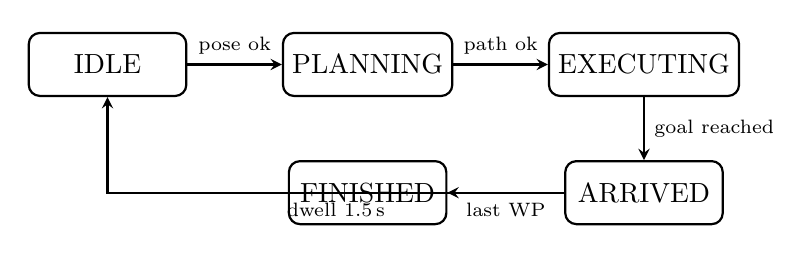
\begin{tikzpicture}[
    state/.style={draw,thick,rounded corners,minimum width=2cm,minimum height=0.8cm,align=center,fill=white},
    arr/.style={-stealth,thick},
    scale=1.0
  ]
    \node[state] (idle) {IDLE};
    \node[state, right=1.2cm of idle] (plan) {PLANNING};
    \node[state, right=1.2cm of plan] (exec) {EXECUTING};
    \node[state, below=0.8cm of exec] (arr) {ARRIVED};
    \node[state, below=0.8cm of plan] (fin) {FINISHED};

    \draw[arr] (idle) -- node[above,font=\scriptsize] {pose ok} (plan);
    \draw[arr] (plan) -- node[above,font=\scriptsize] {path ok} (exec);
    \draw[arr] (exec) -- node[right,font=\scriptsize] {goal reached} (arr);
    \draw[arr] (arr) -| node[below,font=\scriptsize,pos=0.25] {dwell 1.5\,s} (idle);
    \draw[arr] (arr) -- node[below,font=\scriptsize] {last WP} (fin);
  \end{tikzpicture}

  \medskip
  \small
  \textbf{IDLE} $\to$ wait for first pose. \quad
  \textbf{PLANNING} $\to$ run A\textsuperscript{*} + smooth + arm tracker. \\
  \textbf{EXECUTING} $\to$ Pure Pursuit publishes \texttt{cmd\_vel} at 30\,Hz. \\
  \textbf{ARRIVED} $\to$ stop, dwell, advance to next waypoint. \\
  \textbf{FINISHED} $\to$ closed loop done, brake \& hold.
\end{frame}

% =====================================================================
\section{Results}

\begin{frame}{Part 1 — EKF metrics}
  \begin{columns}[T,onlytextwidth]
    \column{0.5\textwidth}
    \textbf{Localization accuracy} \\
    Trajectory averaged over the maze loop, against \texttt{/ground\_truth}:
    \medskip
    \begin{tabular}{lr}
      \toprule
      Metric & Value \\
      \midrule
      RMSE position & $\approx 7$\,mm \\
      Detection rate & $99\%$ \\
      NEES in band & $87.5\%$ \\
      Mahalanobis rejects & $< 5\%$ \\
      \bottomrule
    \end{tabular}

    \medskip
    NEES band: $\chi^2_{2,\,0.025} \leq \mathrm{NEES} \leq \chi^2_{2,\,0.975}$
    \\ $\Rightarrow$ filter is statistically consistent.

    \column{0.45\textwidth}
    \textbf{What the demo shows}
    \begin{itemize}
      \item Covariance ellipse \emph{breathes} as markers come into view.
      \item No marker visible $\Rightarrow$ ellipse \textbf{grows}.
      \item ArUco update lands $\Rightarrow$ ellipse \textbf{shrinks}.
      \item Trail of past ellipses traces the uncertainty history along
            the path.
    \end{itemize}
  \end{columns}
\end{frame}

% =====================================================================
\begin{frame}{Part 2 — Navigation result}
  \begin{columns}[T,onlytextwidth]
    \column{0.55\textwidth}
    \textbf{Closed trajectory completed:}
    \[
      p_0 \to p_1 \to p_2 \to p_3 \to p_0
    \]
    Heading change at every leg $> 50^\circ$ (PDF requirement: no two
    consecutive co-directional legs). The robot circumnavigates all four
    inner chambers.

    \medskip
    \textbf{No collisions.} The configuration-space inflation
    ($r = 0.28\,\text{m}$) guarantees every A\textsuperscript{*} path stays
    $\geq 28\,$cm from any wall, even with EKF drift.

    \medskip
    \textbf{Pipeline runs from scratch}: A\textsuperscript{*}, Catmull-Rom,
    Pure Pursuit, EKF — all implemented with NumPy only.

    \column{0.4\textwidth}
    \centering
    \scriptsize
    \begin{tabular}{lr}
      \toprule
      Property & Value \\
      \midrule
      Lap time & $\approx 75$\,s \\
      Max speed $v_{\max}$ & $0.18$\,m/s \\
      Max angular $\omega_{\max}$ & $0.8$\,rad/s \\
      Lookahead $L_d$ & $0.30$\,m \\
      Grid resolution & $0.05$\,m \\
      Robot radius (C-space) & $0.28$\,m \\
      Control rate & $30$\,Hz \\
      Planning rate & $1$\,Hz \\
      \bottomrule
    \end{tabular}
  \end{columns}
\end{frame}

% =====================================================================
\begin{frame}{Why this satisfies the PDF rubric}
  \begin{itemize}
    \item \textbf{Part 1}: EKF with prediction, ArUco-based update,
          confidence ellipses, three PDF scenarios (multi / no / partial marker)
          — \checkmark
    \item \textbf{Part 2}: 4 waypoints, closed trajectory, no straight legs,
          no co-directional consecutive legs, circumnavigates obstacles
          — \checkmark
    \item \textbf{Optional A}: global planner with A\textsuperscript{*}
          + spline smoothing instead of pure reactive — \checkmark
    \item \textbf{Optional B}: EKF runs in parallel during navigation
          and is plotted in RViz with the covariance ellipse — \checkmark
    \item \textbf{Library constraint}: only NumPy + Python stdlib, no scipy,
          no Nav2, no SLAM toolbox — \checkmark
  \end{itemize}
\end{frame}

% =====================================================================
\begin{frame}[fragile]{Live demo plan}
  \small
  \textbf{Timeline of the recorded video:}
  \begin{enumerate}
    \item \textbf{0–10\,s} — overview: RViz + Gazebo side by side.
    \item \textbf{10–30\,s} — Part 1 in action: zoom on the covariance ellipse,
          show how it shrinks when an ArUco lands and grows on long stretches.
    \item \textbf{30–75\,s} — Part 2 timelapse ($\times$4): robot completes the
          full $p_0 \to p_1 \to p_2 \to p_3 \to p_0$ loop, planner path
          visible in green, LiDAR sweep visible in red.
    \item \textbf{75–90\,s} — final frame: \emph{Mission complete}, robot
          stops at the closing waypoint.
  \end{enumerate}

  \medskip
  Reproduce with:
  \begin{lstlisting}[language=bash,basicstyle=\ttfamily\scriptsize]
./run.sh part2-astar
  \end{lstlisting}
\end{frame}

% =====================================================================
\begin{frame}
  \vfill
  \centering
  {\Huge\bfseries Thank you}\\[1em]
  {\large Alfonso Diaz}\\[0.3em]
  \texttt{personaldiaz01@gmail.com}\\[2em]
  \footnotesize
  Code: \texttt{challenges/Week7/Challenge/}\\
  Run with \texttt{./run.sh part2-astar}\\[1em]
  \textcolor{black!50}{MCR2 × NVIDIA · TE3003B · 2026}
  \vfill
\end{frame}

\end{document}
